\documentclass[a4paper,12pt]{article}

\usepackage[utf8]{inputenc}
\usepackage{geometry}
\usepackage{graphicx}
\usepackage{amsmath}
\usepackage{hyperref}

\geometry{margin=1in}

\title{Algorithm PA2 report}
\author{Ivan Chang}
\date{\today}

% Language and font packages
% \usepackage{ctex} % Chinese support

% Pseudocode and algorithm packages
\usepackage{algorithm2e} % Advanced algorithm writing
\usepackage{algpseudocode} % Pseudocode environment for algorithms

% Fancy style packages
\usepackage{fancyhdr} % Custom headers/footers
\usepackage{color} % Color support
\usepackage{xcolor} % Extended color support
\usepackage{tcolorbox} % Colored boxes
\usepackage{framed} % Framed environments

% Math and symbol packages
\usepackage{amsfonts}
\usepackage{amssymb}
\usepackage{mathtools}

% Table and figure packages
\usepackage{booktabs} % Professional tables
\usepackage{multirow} % Multi-row tables
\usepackage{caption} % Custom captions
\usepackage{subcaption} % Subfigures

% Miscellaneous
\usepackage{enumitem} % Custom lists
\usepackage{listings} % Code listings
\usepackage{tikz} % Drawing diagrams
\usepackage{pgfplots} % For plotting graphs
\usepackage{float}

\begin{document}

\maketitle

\section{Data Structure}
\begin{itemize}
\item \textbf{vector}: vector is a dynamic array which supports allocating memory dynamically. In my assignment, 
I use vector to store the dp value. 
\item \textbf{pair}: pair is a data sturcture which can pair two values(whether or not they are the same format)
in my assignment, I use it to represent the chords. For chord ij, I store it as (min(i,j), max(i,j))
\end{itemize}

\section{Method Output}
\begin{figure}[H]
    \centering
    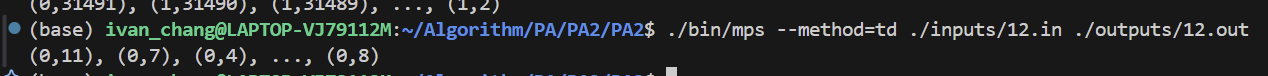
\includegraphics[width=0.8\textwidth]{method_td.png}
    \caption{Output for td method}
    \label{fig:method_output_td}
\end{figure}    
\begin{figure}[H]
    \centering
    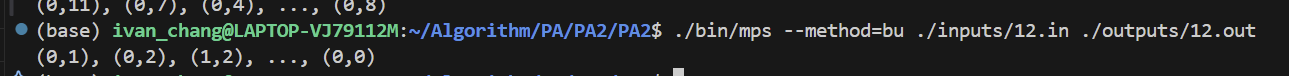
\includegraphics[width=0.8\textwidth]{method_bu.png}
    \caption{Output for bu method}
    \label{fig:method_output_bu}
\end{figure}
\section{Result Analysis}
I have run my code on edaunion server. and iterate through all the test case from {12, 1000, 10000, 20000, 40000, 60000, 80000, 100000, 120000, 180000}
Below are the times required and the memory used for each test case.
\begin{figure}[H]
    \centering
    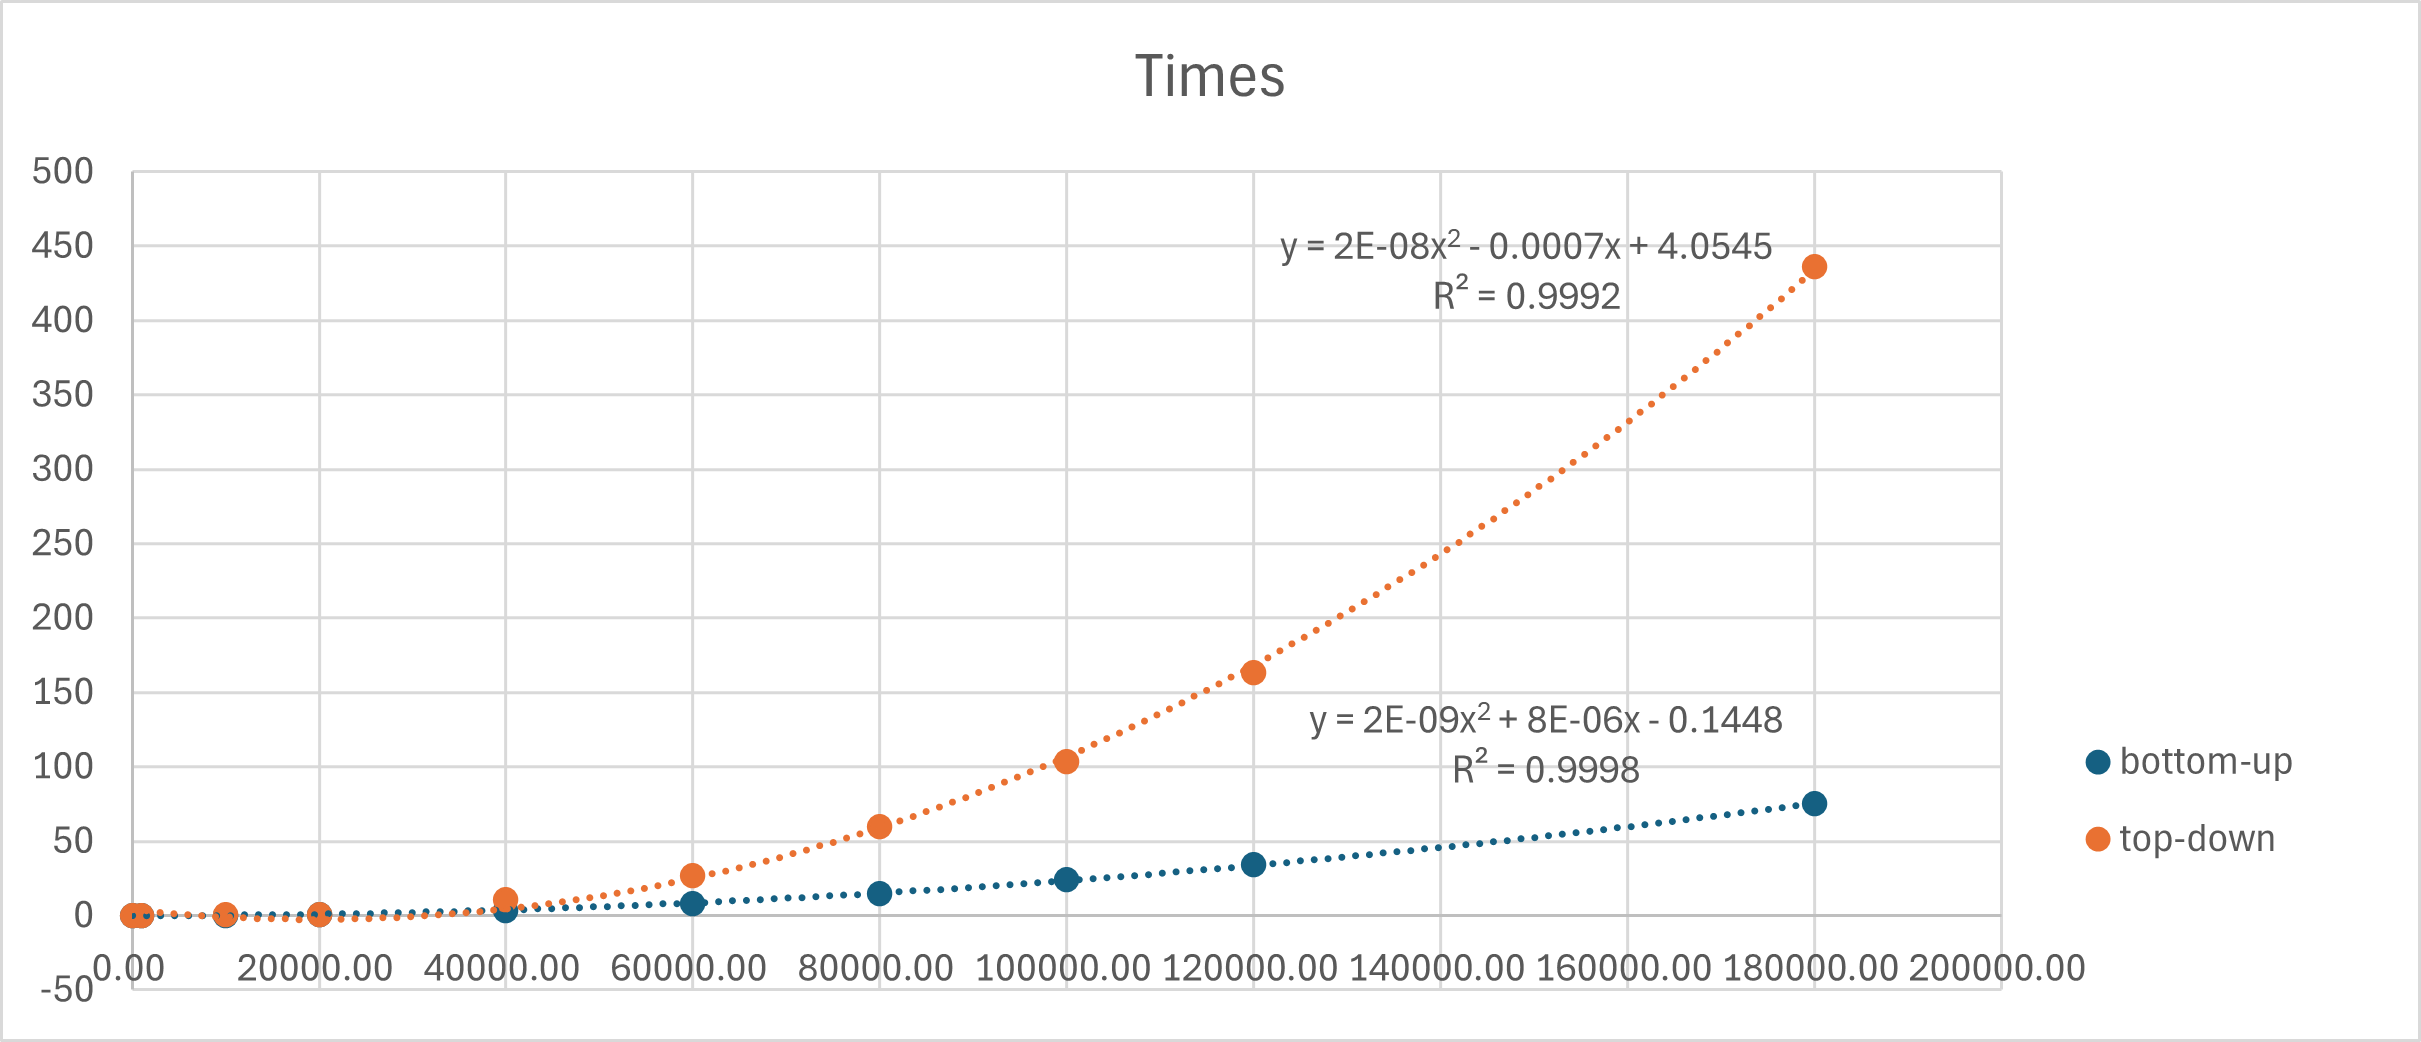
\includegraphics[width=0.8\textwidth]{time_result.png}
    \caption{Time vs Input Size}
    \label{fig:time_plot}
\end{figure}
\begin{figure}[H]
    \centering
    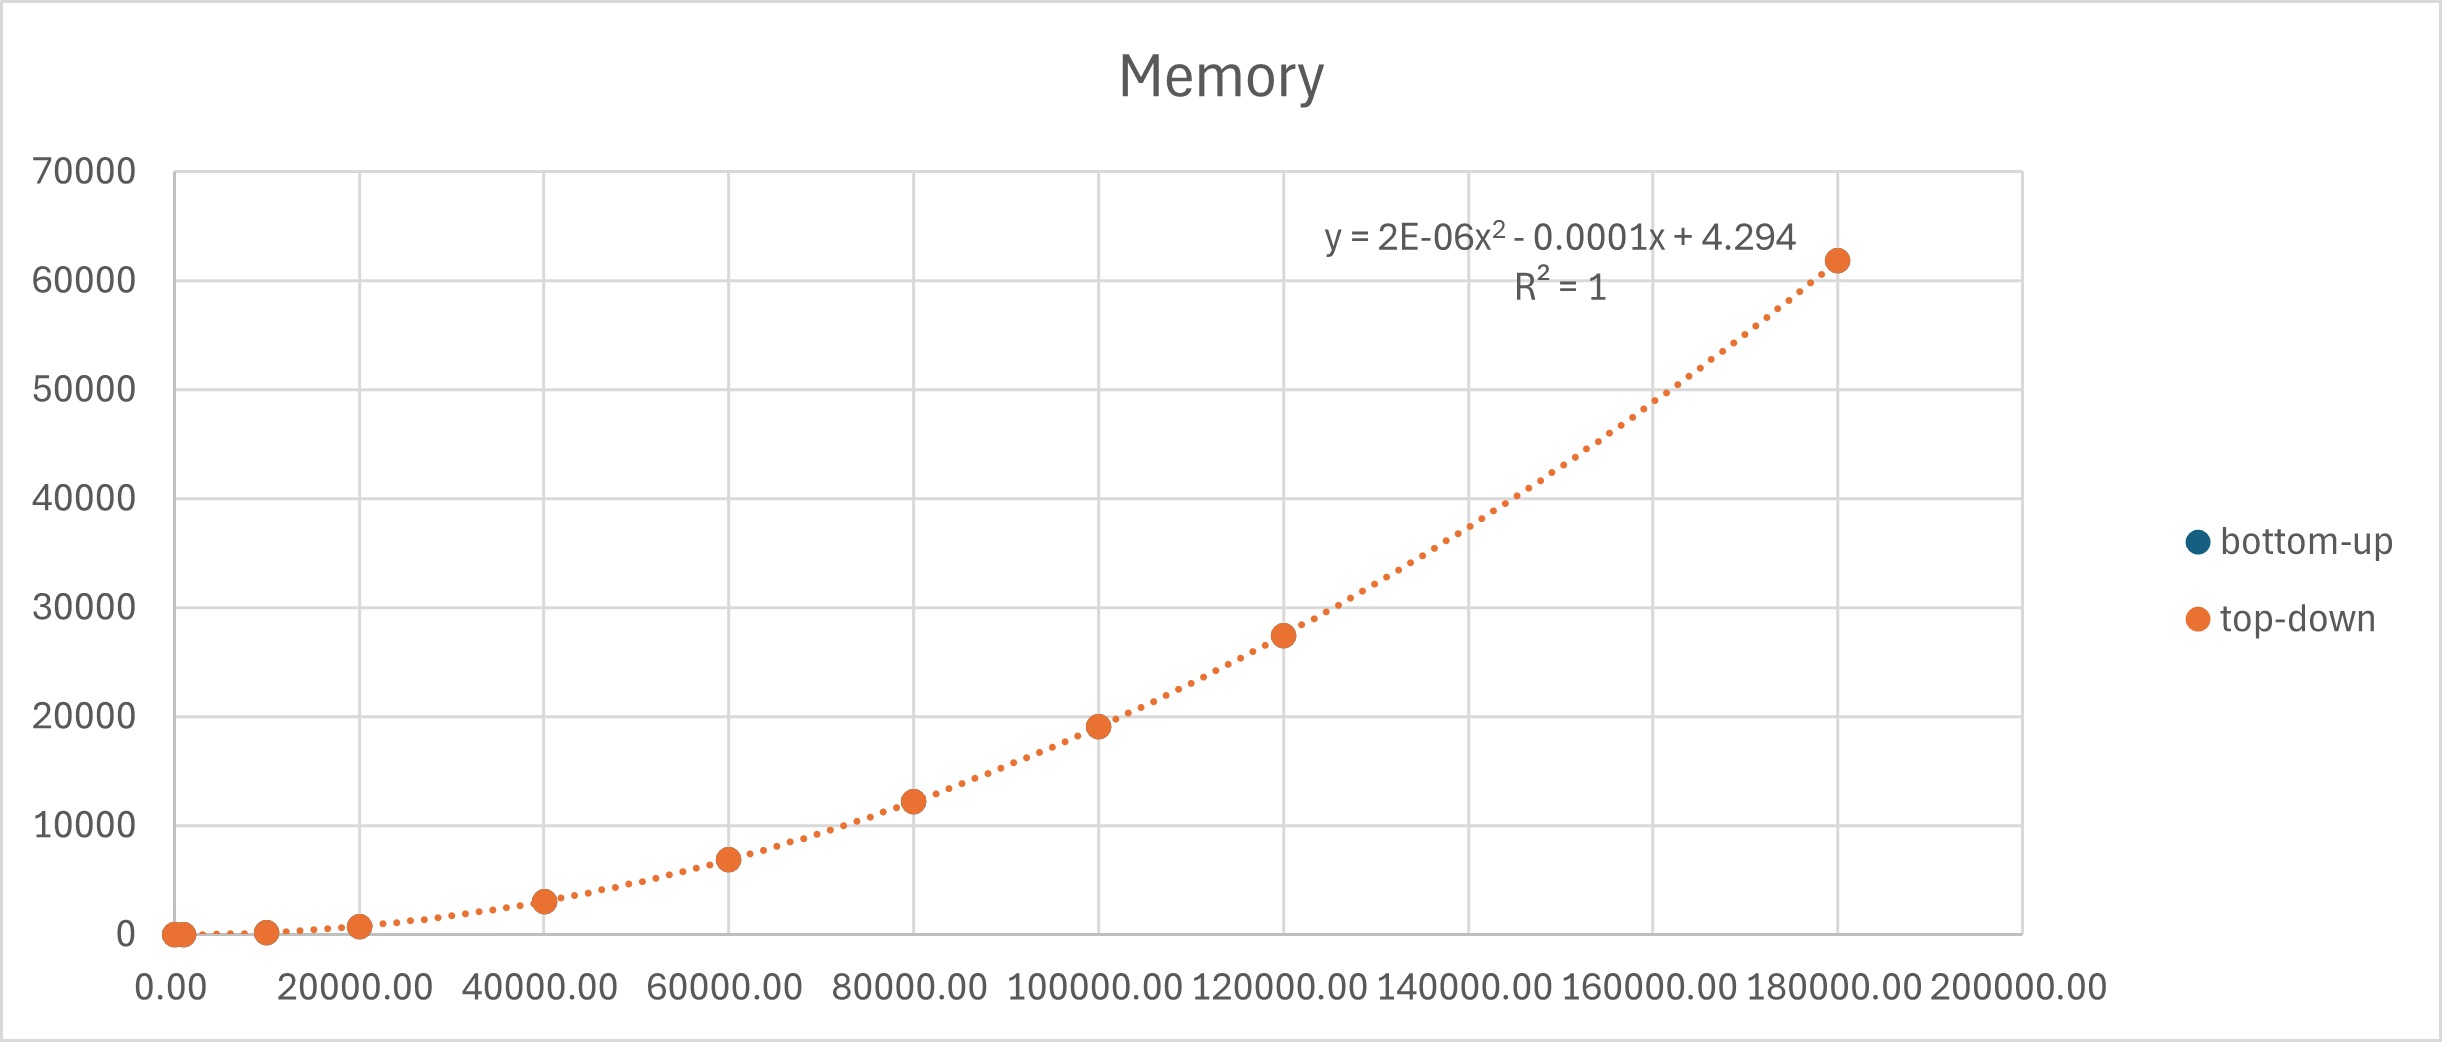
\includegraphics[width=0.8\textwidth]{memory_result.png}
    \caption{Memory vs Input Size}
    \label{fig:memory_plot}
\end{figure}
\subsection{discussion}
\begin{itemize}
    \item From figure \ref{fig:memory_plot}, we can see that the space complexity is $O(n^2)$ since we open a triangular 2D array to store the dp value.
    \item From figure \ref{fig:time_plot}, we can see that the time complexity is also $O(n^2)$, which is expected since we need to fill in the 2D dp array.
    \item bottom-up method is faster than top-down method. This is because in bottom-up method, we do not have the overhead of recursive function calls. and the cache issue is solved through my adjustment.
\end{itemize}

\section{Other Findings}
\begin{enumerate}
    \item the max input size is 180000. Since each int value takes 4 bytes. We need $180000*180000*4 \approxeq 129GB$ 
    which is far beyond the memory limit. However, we notice that i <= j for all cases. which implys that we only need $\frac{2n*2n+1}{2}$ spaces for storage.
    It can reduce the size by half. 
    \item For bottom-up dp, the iteraration order matters. Instead of iterating l to i, we have to iterate from j to i. This is because of the performance of the cache.
    when we access memory, the cache will load a block of memory into the cache line. Through my adjestment, the hit rate of cache is improved significantly. So the speed of 
    my bottom-up method is improved.
\end{enumerate}


\end{document}